\documentclass[dvipdfmx,a4paper,11pt]{article}
\usepackage[utf8]{inputenc}
%\usepackage[dvipdfmx]{hyperref} %リンクを有効にする
\usepackage{url} %同上
\usepackage{amsmath,amssymb} %もちろん
\usepackage{amsfonts,amsthm,mathtools} %もちろん
\usepackage{braket,physics} %あると便利なやつ
\usepackage{bm} %ラプラシアンで使った
\usepackage[top=30truemm,bottom=30truemm,left=25truemm,right=25truemm]{geometry} %余白設定
\usepackage{latexsym} %ごくたまに必要になる
\renewcommand{\kanjifamilydefault}{\gtdefault}
\usepackage{otf} %宗教上の理由でmin10が嫌いなので


\usepackage[all]{xy}
\usepackage{amsthm,amsmath,amssymb,comment}
\usepackage{amsmath}    % \UTF{00E6}\UTF{0095}°\UTF{00E5}\UTF{00AD}\UTF{00A6}\UTF{00E7}\UTF{0094}¨
\usepackage{amssymb}  
\usepackage{color}
\usepackage{amscd}
\usepackage{amsthm}  
\usepackage{wrapfig}
\usepackage{comment}	
\usepackage{graphicx}
\usepackage{setspace}
\setstretch{1.2}


\newcommand{\R}{\mathbb{R}}
\newcommand{\Z}{\mathbb{Z}}
\newcommand{\N}{\mathbb{N}}
\newcommand{\C}{\mathbb{C}} 
\newcommand{\Area}{\text{Area}}





   %当然のようにやる.
\allowdisplaybreaks[4]
   %もちろん.
%\title{第1回. 多変数の連続写像 (岩井雅崇, 2020/10/06)}
%\author{岩井雅崇}
%\date{2020/10/06}
%ここまで今回の記事関係ない
\usepackage{tcolorbox}
\tcbuselibrary{breakable, skins, theorems}

\theoremstyle{definition}
\newtheorem{thm}{定理}
\newtheorem{lem}[thm]{補題}
\newtheorem{prop}[thm]{命題}
\newtheorem{cor}[thm]{系}
\newtheorem{claim}[thm]{主張}
\newtheorem{dfn}[thm]{定義}
\newtheorem{rem}[thm]{注意}
\newtheorem{exa}[thm]{例}
\newtheorem{conj}[thm]{予想}
\newtheorem{prob}[thm]{問題}
\newtheorem{rema}[thm]{補足}

\DeclareMathOperator{\Ric}{Ric}
\DeclareMathOperator{\Vol}{Vol}
 \newcommand{\pdrv}[2]{\frac{\partial #1}{\partial #2}}
 \newcommand{\drv}[2]{\frac{d #1}{d#2}}
  \newcommand{\ppdrv}[3]{\frac{\partial #1}{\partial #2 \partial #3}}


%ここから本文.
\begin{document}
%\maketitle
\begin{center}
{\Large 第13回. 線積分とグリーンの定理  (川平先生の本, 第11・29章の内容)}
\end{center}

\begin{flushright}
 岩井雅崇, 2021/01/19
\end{flushright}


\section{はじめに}
第13回と第14回はベクトル解析の初歩(イントロ)に関する授業を行う.
授業準備のために, 以下の文献も参考した.
\begin{itemize}
\item 川平友規先生 解析学概論第三第四(ベクトル解析) available at \url{http://www.math.titech.ac.jp/~kawahira/courses/17W-kaiseki.html}
\end{itemize}
時々この文献を引用する.(引用する際は"川平先生のpdf"と呼ぶことにする.)

他にも第14回の資料の最後に参考文献を書いておいたので, 必要であれば見てほしい.

\section{線積分}


 \begin{tcolorbox}[
    colback = white,
    colframe = green!35!black,
    fonttitle = \bfseries,
    breakable = true]
    \begin{dfn}
    
  $D \subset \R^2$を領域とする.
  $u(x,y), v(x,y)$を$D$上の$C^n$級関数として, 
 $$
\begin{array}{ccccc}
V: &D & \rightarrow & \R^2 & \\
&(x,y) & \longmapsto & (u(x,y), v(x,y))&
\end{array}
$$
となる(ベクトル値の)関数$V$を\underline{$D$上の$C^n$級ベクトル場}という. 

 \end{dfn}
 \end{tcolorbox}
 
 \begin{exa}
 $\R^2$上のベクトル場$V(x,y)=(-y,x)$を考えると, これは反時計回りの渦まきの形になっている.
 \end{exa}
 
  \begin{tcolorbox}[
    colback = white,
    colframe = green!35!black,
    fonttitle = \bfseries,
    breakable = true]
    \begin{dfn}
    \text{}
    
    \begin{itemize}
\item 関数 $\vec{p}(t)$ を次で定める.
$$
\begin{array}{ccccc}
\vec{p}: &[a,b] & \rightarrow & \R^2 & \\
&t & \longmapsto &\vec{p}(t) = (x(t), y(t))&
\end{array}
$$
関数 \underline{$\vec{p}(t)$が滑らかな曲線}とは次の2条件を満たすこと.
\begin{enumerate}
\item[条件1.] $x(t),y(t)$が$C^1$級.
\item[条件2.]  任意の$c \in (a,b)$について, 速度ベクトル$\drv{\vec{p}}{t}(c)=\left( \drv{x}{t}(c),\drv{y}{t}(c)  \right)$がゼロベクトル$\vec{0} = (0,0)$ではない.
\end{enumerate}
%$x(t),y(t)$が$C^1$級であり, 任意の$c \in (a,b)$について, 速度ベクトル$\drv{\vec{p}}{t}(c)=\left( \drv{x}{t}(c),\drv{y}{t}(c)  \right)$がゼロベクトル$\vec{0} = (0,0)$ではないこと.
\item \underline{曲線$C: \vec{p}(t) (a \leqq t \leqq b)$が区分的に滑らかな曲線}とは
滑らかな曲線を端点でつないだもの.
%$x(t),y(t),z(t)$が$C^1$級であり, 有限個の$c \in (a,b)$を除いて, 速度ベクトル$\drv{\vec{p}}{t}(c)=\left( \drv{x}{t}(c),\drv{y}{t}(c), \drv{z}{t}(c) \right)$がゼロベクトル$\vec{0}$ではないこと.

\end{itemize}
     \end{dfn}
 \end{tcolorbox}
 \footnote{"曲線$C: \vec{p}(t) (a \leqq t \leqq b)$が区分的に滑らかな曲線"という定義を厳密にいうなら,「有限個の$c \in (a,b)$を除いて, $x(t),y(t)$が$C^1$級であり,速度ベクトル$\drv{\vec{p}}{t}(t)=\left( \drv{x}{t}(t),\drv{y}{t}(t) \right)$がゼロベクトル$\vec{0}$ではない」.}
 
  \begin{exa}
円周は滑らかな曲線であり, 長方形の周は区分的に滑らかな曲線である.
 \end{exa}
 
 
  \begin{tcolorbox}[
    colback = white,
    colframe = green!35!black,
    fonttitle = \bfseries,
    breakable = true]
    \begin{dfn}
  $D \subset \R^2$を領域とし, $D$上の$C^1$級ベクトル場を$V(x,y)=(u(x,y),v(x,y))$とする. 
  $D$内の滑らかな曲線$C: \vec{p}(t) (a \leqq t \leqq b)$について
\underline{$V$の曲線$C$に沿った線積分}を

 
   
\begin{align*}
\begin{split}
\int_{C}V(\vec{p}) d\vec{p} &= \int_{a}^{b}\left( V(\vec{p}(t)) \cdot \drv{\vec{p}}{t} \right)dt \\
&=\int_{a}^{b} \left( u(x(t),y(t))\cdot \drv{x}{t}+v(x(t),y(t))\cdot \drv{y}{t}  \right) dt \text{\,\,とする.}
\end{split}
\end{align*}
この線積分$\int_{C}V(\vec{p}) d\vec{p} $を$\int_{C}udx+vdy$と書くこともある.



 \end{dfn}
 \end{tcolorbox}
 \footnote{線積分$\int_{C}V(\vec{p}) d\vec{p} $を$\int_{C}udx+vdy$と書くのは, (向きを込めた場合)この積分がパラメーターの取り方に寄らないからである. 詳しくは川平先生のpdfの命題4.2を参照せよ. (連鎖律からすぐに分かるのだが...)}

 
 \begin{exa}
 $C^1$級ベクトル場$V(x,y)=(2x,2y)$とし, 滑らかな曲線$C: \vec{p}(t)=(t,t^2) (0 \leqq t \leqq 1)$とする.
 $V$の$C$に沿った線積分$\int_{C}V(\vec{p}) d\vec{p} =\int_{C}2xdx+2ydy$の値を求めよ.
 
 \hspace{-11pt}(解.)
 $V(\vec{p}(t)) = (2t,2t^2)$かつ$\drv{\vec{p}}{t} = (1,2t)$より, 
$$
\int_{C}2xdx+2ydy=\int_{C}\left( V(\vec{p}(t)) \cdot \drv{\vec{p}}{t} \right)dt  =\int_{0}^{1} (2t\cdot1+2t^2\cdot2t)dt
=\int_{0}^{1}(2t+4t^3)dt=2.
$$
 \end{exa}
 
  \begin{exa}[ハイキングの原理] 
   $D \subset \R^2$を領域とし. 
  $F(x,y): D \rightarrow \R$を$C^1$級関数とする. \\
  \underline{勾配ベクトル場を$\nabla F =\left(\pdrv{F}{x},\pdrv{F}{y} \right)$と定める.}
  $D$内の滑らかな曲線$C: \vec{p}(t) (a \leqq t\leqq b)$とするとき
$$
  \int_{C}\nabla F(\vec{p}) d\vec{p}
  =\int_{a}^{b}\left( \pdrv{F}{x}\drv{x}{t}+\pdrv{F}{y}\drv{y}{t} \right)dt
  =\int_{a}^{b}\drv{F}{t}(\vec{p}(t))dt
  =F(\vec{p}(b))-F(\vec{p}(a)).
$$
つまり, $\vec{\alpha}=\vec{p}(a)$, $\vec{\beta}=\vec{p}(b)$とおくと, 
$
  \int_{C}\nabla F(\vec{p}) d\vec{p}=F(\vec{\beta})-F(\vec{\alpha})\text{\,\,である.}
$
  \end{exa}


\section{グリーンの定理}
  \begin{tcolorbox}[
    colback = white,
    colframe = green!35!black,
    fonttitle = \bfseries,
    breakable = true]
    \begin{dfn}
   $\R^2$内の区分的に滑らかな曲線$C: \vec{p}(t) (a \leqq t\leqq b)$が\underline{単純閉曲線}とは次の二つの条件を満たすこと.
   \begin{enumerate}
   \item[条件1.] 始点と終点が一致する.(つまり$\vec{p}(a)=\vec{p}(b)$.)
   \item[条件2.] 自己交差しない.(つまり$a<s<t<b$なる$s,t$について$\vec{p}(s)\neq \vec{p}(t)$.)
   \end{enumerate}


 \end{dfn}
 \end{tcolorbox}
 
 
   \begin{tcolorbox}[
    colback = white,
    colframe = green!35!black,
    fonttitle = \bfseries,
    breakable = true]
    \begin{thm}[グリーンの定理]
 $\R^2$内の単純閉曲線$C: \vec{p}(t)=(x(t), y(t)) (a \leqq t\leqq b)$について$D \subset \R^2$を$C$で囲まれる有界な閉集合とする.
 $C$の進行方向の左側に$D$があると仮定する.
 
 $D$を含む開集合上で定義された$C^1$級ベクトル場$V(x,y)=(u(x,y) , v(x,y))$について以下が成り立つ.
 $$
 \int_{C}V(\vec{p}) d\vec{p} =\int_{C}udx+vdy
 =\iint_{D}\left(\pdrv{v}{x} - \pdrv{u}{y} \right)dxdy
 $$

 $$
\text{特に}
\Area(D)=\int_{C}xdy=\int_{C}-ydx \text{\,\,が成り立つ.} 
 $$
 \end{thm}
 \end{tcolorbox}
 
 \begin{wrapfigure}{r}[5pt]{0.25\textwidth}
  \centering
 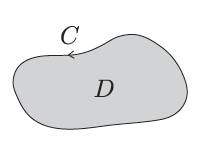
\includegraphics[height=25mm, width=35mm]{green.jpg}
 %\caption{キャプション。}
\end{wrapfigure}
 $D \subset \R^2$を$C$で囲まれる有界閉集合および, $C$の進行方向の左側に$D$があるとは右の図のようなことが成り立つことである
 
 
\begin{exa}
$C:\vec{p}(t)=(\cos t , \sin t) (0\leqq t \leqq 2\pi)$とし, $\R^2$上のベクトル場$V(x,y)=(x^2-y^2,-2xy)$とする. \\
線積分$ \int_{C}V(\vec{p}) d\vec{p} = \int_{C}(x^2-y^2)dx-2xydy$を求めよ.

\hspace{-11pt}(解.)普通に計算すると, 
\begin{align*}
\begin{split}
\int_{C}V(\vec{p}) d\vec{p}  
&= \int_{0}^{2\pi} \left \{(\cos^2 t - \sin^2 t)\drv{x}{t}-(2\sin t \cos t) \drv{y}{t} \right \} dt \\
&=\int_{0}^{2\pi} \left \{ -\cos^2 t \sin t + \sin^3 t -2\sin t \cos^2 t  \right\}dt
= \text{(計算略)}
= 0
\end{split}
\end{align*}

グリーンの定理を使う方法は以下のようになる.

$C$で囲まれた領域$D$とすると, $D$は原点中心の半径1の円である.
$V(x,y)=(u(x,y) , v(x,y))=(x^2-y^2,-2xy)$は$D$を含む開集合上で定義された$C^1$級ベクトル場である.\footnote{今回は$D$を含む開集合として$\R^2$が取れる.}
よってグリーンの定理の仮定を満たす.
$$
\pdrv{v}{x}=\pdrv{(-2xy)}{x}=-2y, \text{\,\,} \pdrv{u}{y}=\pdrv{(x^2-y^2)}{y}=-2y \text{\,\,であるため, }
$$
$$
\int_{C}(x^2-y^2)dx-2xydy =\iint_{D}\left(\pdrv{v}{x} - \pdrv{u}{y} \right)dxdy = \iint_{D}\left(-2y + 2y \right)dxdy =0.
$$
\end{exa}

\begin{exa}
$a,b$を正の数として, 楕円$D$を下で定める.
$$D = \left\{ (x,y) \in \R^2 : \frac{x^2}{a^2}+\frac{y^2}{b^2} \leqq 1 \right\}
=\left\{ (x,y) \in \R^2 :  -a \leqq x \leqq a, -b\sqrt{1-\frac{x^2}{a^2}} \leqq y \leqq b\sqrt{1-\frac{x^2}{a^2}} \right\}.
$$
$D$の面積$\Area(D)$を求めよ.

\hspace{-11pt}(解.)普通に計算すると, 
\begin{align*}
\begin{split}
\Area(D)=\int_{D}dxdy
= \int_{-a}^{a} \left( b\sqrt{1-\frac{x^2}{a^2}}-(-b)\sqrt{1-\frac{x^2}{a^2}}\right) dx =\int_{-a}^{a} 2 b\sqrt{1-\frac{x^2}{a^2}} dx =\text{(計算略)} = \pi ab.
\end{split}
\end{align*}

グリーンの定理を使うと以下の通りになる.
$C :\vec{p}(t) = (a \cos t, b \sin t) (0 \leqq t \leqq 2\pi)$と置けば,
楕円$D$は$C$で囲まれた領域となる.
よってグリーンの定理が使えて, $\drv{y}{t} = b \cos t$のため, 
$$
\Area(D)=\int_{C}xdy=\int_{0}^{2\pi} a \cos t \drv{y}{t} dt
= \int_{0}^{2\pi} ab \cos^2 t  dt = \pi ab.
$$
となる. (どちらが楽かは皆さんに委ねます.)
\end{exa}

 
 
\end{document}
